---
id: tkz-euclide-ejemplo-64
title: "Modelando la Pirámide de Giza"
description: "Modelado de diagramas con gráficos"
keywords: [taller5,graficos,modelado]
tags: [tkzClip,node,includegraphics,tkzDrawPolySeg,tkzDefParallelogram,tkzInterLL,tkzMarkRightAngle]
sort: 64
---
\documentclass[tikz,border=2mm]{standalone}
\usepackage{graphicx}
\usepackage{xcolor}
\usepackage{tkz-base}
\usepackage{tkz-euclide}

\begin{document}    
    \begin{tikzpicture}[dim style/.style={dashed,sloped,Triangle-Triangle}]
        
        % Paso 1: Definir plano de coordenadas
        \tkzInit[xmin=0,xmax=16,ymin=0,ymax=15]        

        % Paso 2: Corta el plano para que no exceda las coordenadas
        \tkzClip

        % Paso 3: Carga imagen de la Pirámide de Giza en el plano
        % en el punto (13,7.5) con opacidad del 50% a escala del 50%
         \node[opacity=0.5] at (13,7.5){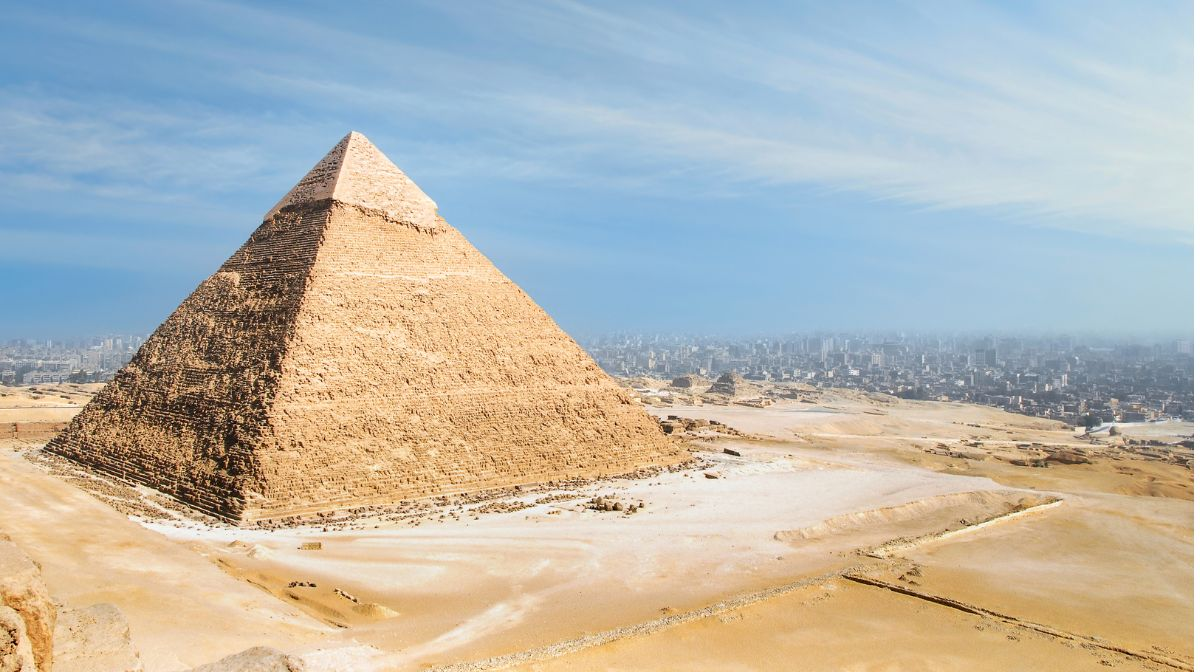
\includegraphics[scale=0.5]{piramide-giza.jpg}};

        % Paso 4: Coloca título sobre la imagen
        \tkzText[font=\Large](4,13.5){\textbf{Pirámide de Giza}}
        
        % Paso 5: Define los puntos de la pirámide V-ABC
        \tkzDefPoints{
            7.6  /12   /V,
            0.8  /5.0  /A,
            5.0  /3.3  /B,
            15   /5.0  /C% 
        }

        % Paso 6: Etiqueta los puntos en posiciones clave
        \tkzLabelPoints[left](A)
        \tkzLabelPoints[above right](B)
        \tkzLabelPoints[right](C)
        \tkzLabelPoints[above](V)

        % Paso 7: Dibuja polígonos de la pirámide
        \tkzDrawPolygon[thick](A,B,V)
        \tkzDrawPolygon[thick](B,C,V)

        % Paso 8: Dibuja dimensiones de la base de la pirámide
        \tkzDrawSegment[thick,dim={$230$,-10pt,below=2pt}](A,B)
        \tkzDrawSegment[thick,dim={$230$,-10pt,below=2pt}](B,C)

        % Paso 9: Define el paralelogramo de la base para obtener punto D
        \tkzDefParallelogram(A,B,C) \tkzGetPoint{D}
        \tkzLabelPoints[above right](D)

        % Paso 10: Dibuja líneas punteadas de la base
        \tkzDrawPolySeg[thick,dashed](C,D,A)

        % Paso 11: Encuentra el punto central de la base de la pirámide
        \tkzInterLL(A,C)(B,D) \tkzGetPoint{P}        
        \tkzLabelPoints(P)            

        % Paso 12: Dibuja líneas punteadas del resto de la pirámide
        \tkzDrawSegments[thick,dashed](D,V V,P P,C)

        % Paso 13: Etiqueta el segmento de altura piramidal
        \tkzLabelSegment[right,darkgray!90](P,V){$137$}

        % Paso 14: Marca el ángulo recto de la altura piramidal
        \tkzMarkRightAngle[size=0.5](V,P,C)

        % Paso 15: Marca el ángulo de elevación de la pirámide
        \tkzMarkAngle[size=1.5](V,C,P)
        \tkzLabelAngle(V,C,P){$51^{\circ}$}
    \end{tikzpicture}
\end{document}
